% Ensure included PDFs (banners) with newer versions embed without warnings
\pdfminorversion=7
\documentclass[aspectratio=169]{beamer}

\makeatletter
% Make LaTeX find theme .sty files in Template
\def\input@path{{../Template/}}
\makeatother
\usepackage{graphicx}
% Make graphics (including banner PDFs) resolvable without TEXINPUTS
\graphicspath{{../Template/}{../Template/banners/}{../../Common_Images/}}

%================================================================%
% Theme and Package Setup
%================================================================%
\usetheme{ucl}
\setbeamercolor{banner}{bg=darkpurple}

% Navigation and Footer
\setbeamertemplate{navigation symbols}{\vspace{-2ex}}
\setbeamertemplate{footline}[author title date]
\setbeamertemplate{slide counter}[framenumber/totalframenumber]

\usepackage[utf8]{inputenc}
\usepackage[british]{babel} % British spelling
\usepackage{amsmath, amssymb, amsthm}
\usepackage{graphicx}
\usepackage{tikz}
\usetikzlibrary{calc, positioning, arrows.meta, shapes.geometric, trees, backgrounds, shapes.misc, graphs, quotes, shadows, fit, patterns} 
\usepackage{pgfplots}
\pgfplotsset{compat=1.17}
\usefonttheme{professionalfonts}
\usepackage{eulervm}
\usepackage{listings}
\usepackage{algorithm}
\usepackage{algpseudocode}
\usepackage{xcolor}
\usepackage{subcaption}

% Define custom colours
\makeatletter
\@ifundefined{color@stone}{%
    \definecolor{stone}{gray}{0.95}%
}{}
\makeatother
\definecolor{darkgreen}{rgb}{0.0, 0.5, 0.0}
\definecolor{uclblue}{cmyk}{1,0.24,0,0.64}
\definecolor{uclred}{cmyk}{0,1,0.62,0}

\setbeamercovered{transparent}

% Define theoremblock
\makeatletter
\newenvironment<>{theoremblock}[1]{%
    \begin{block}#2{#1}%
}{\end{block}}
\makeatother

% Section divider slides
\AtBeginSection[]{
  \begin{frame}
    \frametitle{\textbf{\Large\insertsectionhead}}
    \begin{center}
        \huge\textbf{\insertsectionhead}
    \end{center}
  \end{frame}
}

% Maths Macros
\newcommand{\U}{\mathcal{U}}
\newcommand{\V}{\mathcal{V}}
\newcommand{\Z}{\mathcal{Z}}
\newcommand{\R}{\mathbb{R}}
\newcommand{\E}{\mathbb{E}}
\newcommand{\ip}[2]{\langle #1, #2 \rangle}
\newcommand{\norm}[1]{\| #1 \|}
\DeclareMathOperator*{\argmin}{argmin}
\DeclareMathOperator{\prox}{prox}
\DeclareMathOperator{\dom}{dom}
\DeclareMathOperator{\supremum}{sup}
\DeclareMathOperator{\sign}{sign}

\title{Continuous Dynamics and Variational Networks}
\subtitle{Lecture 3: The Early Stopping Paradox and Optimal Control in VNs}
\author[Martin Benning (University College London)]{Martin Benning}
\date[COMP0263]{COMP0263 -- Solving Inverse Problems with Data-Driven Models \\[1cm] 5th March 2026}
\institute[]{University College London}

\begin{document}

% --- Title Frame ---
\begin{frame}
  \titlepage
\end{frame}

% --- Outline ---
\begin{frame}{Lecture Overview}
    \tableofcontents
\end{frame}

\section{The Early Stopping Paradox}

\begin{frame}{A Counter-Intuitive Phenomenon}
    In classic variational image processing, researchers have long observed a counter-intuitive phenomenon:
    
    \vspace{1em}
    \begin{theoremblock}{The Early Stopping Paradox}
    Strictly converging to the global minimum of a regularised energy functional $E(u)$ often yields \textbf{worse} image quality than stopping the iterative minimisation algorithm early \cite{effland2020variational}.
    \end{theoremblock}
    \vspace{1em}
    
    This occurs because even highly expressive, data-driven regularisers cannot perfectly model the true, infinite-dimensional manifold of natural images.
\end{frame}

% \begin{frame}{The Trade-off: Convergence vs. Modelling Errors}
%     There is an inherent trade-off between rigorous mathematical optimisation and modelling errors:
    
%     \begin{itemize}
%         \item \textbf{Initial Iterations:} Iteratively descending the gradient initially removes noise efficiently.
%         \item \textbf{Late Iterations ($t \to \infty$):} As gradient steps continue indefinitely, modelling errors compound. The algorithm begins to destroy true structural image textures.
%     \end{itemize}
%     \vspace{1em}
%     In hand-crafted regularisers like Total Variation (TV-$L^2$), this manifests as artificial ``staircasing'' effects.
% \end{frame}

\begin{frame}{The Trade-off: Convergence vs. Modelling Errors}
    There is an inherent trade-off between rigorous mathematical optimisation and modelling errors.
    
    \begin{columns}[c]
        \begin{column}{0.45\textwidth}
            \begin{itemize}
                \item \textbf{Initial ($t$ is small):} Removes noise efficiently.
                \item \textbf{Late ($t \to \infty$):} Modelling errors compound; destroys true textures (e.g., TV-$L^2$ ``staircasing'').
            \end{itemize}
        \end{column}
        
        \begin{column}{0.55\textwidth}
            \begin{figure}
                \centering
                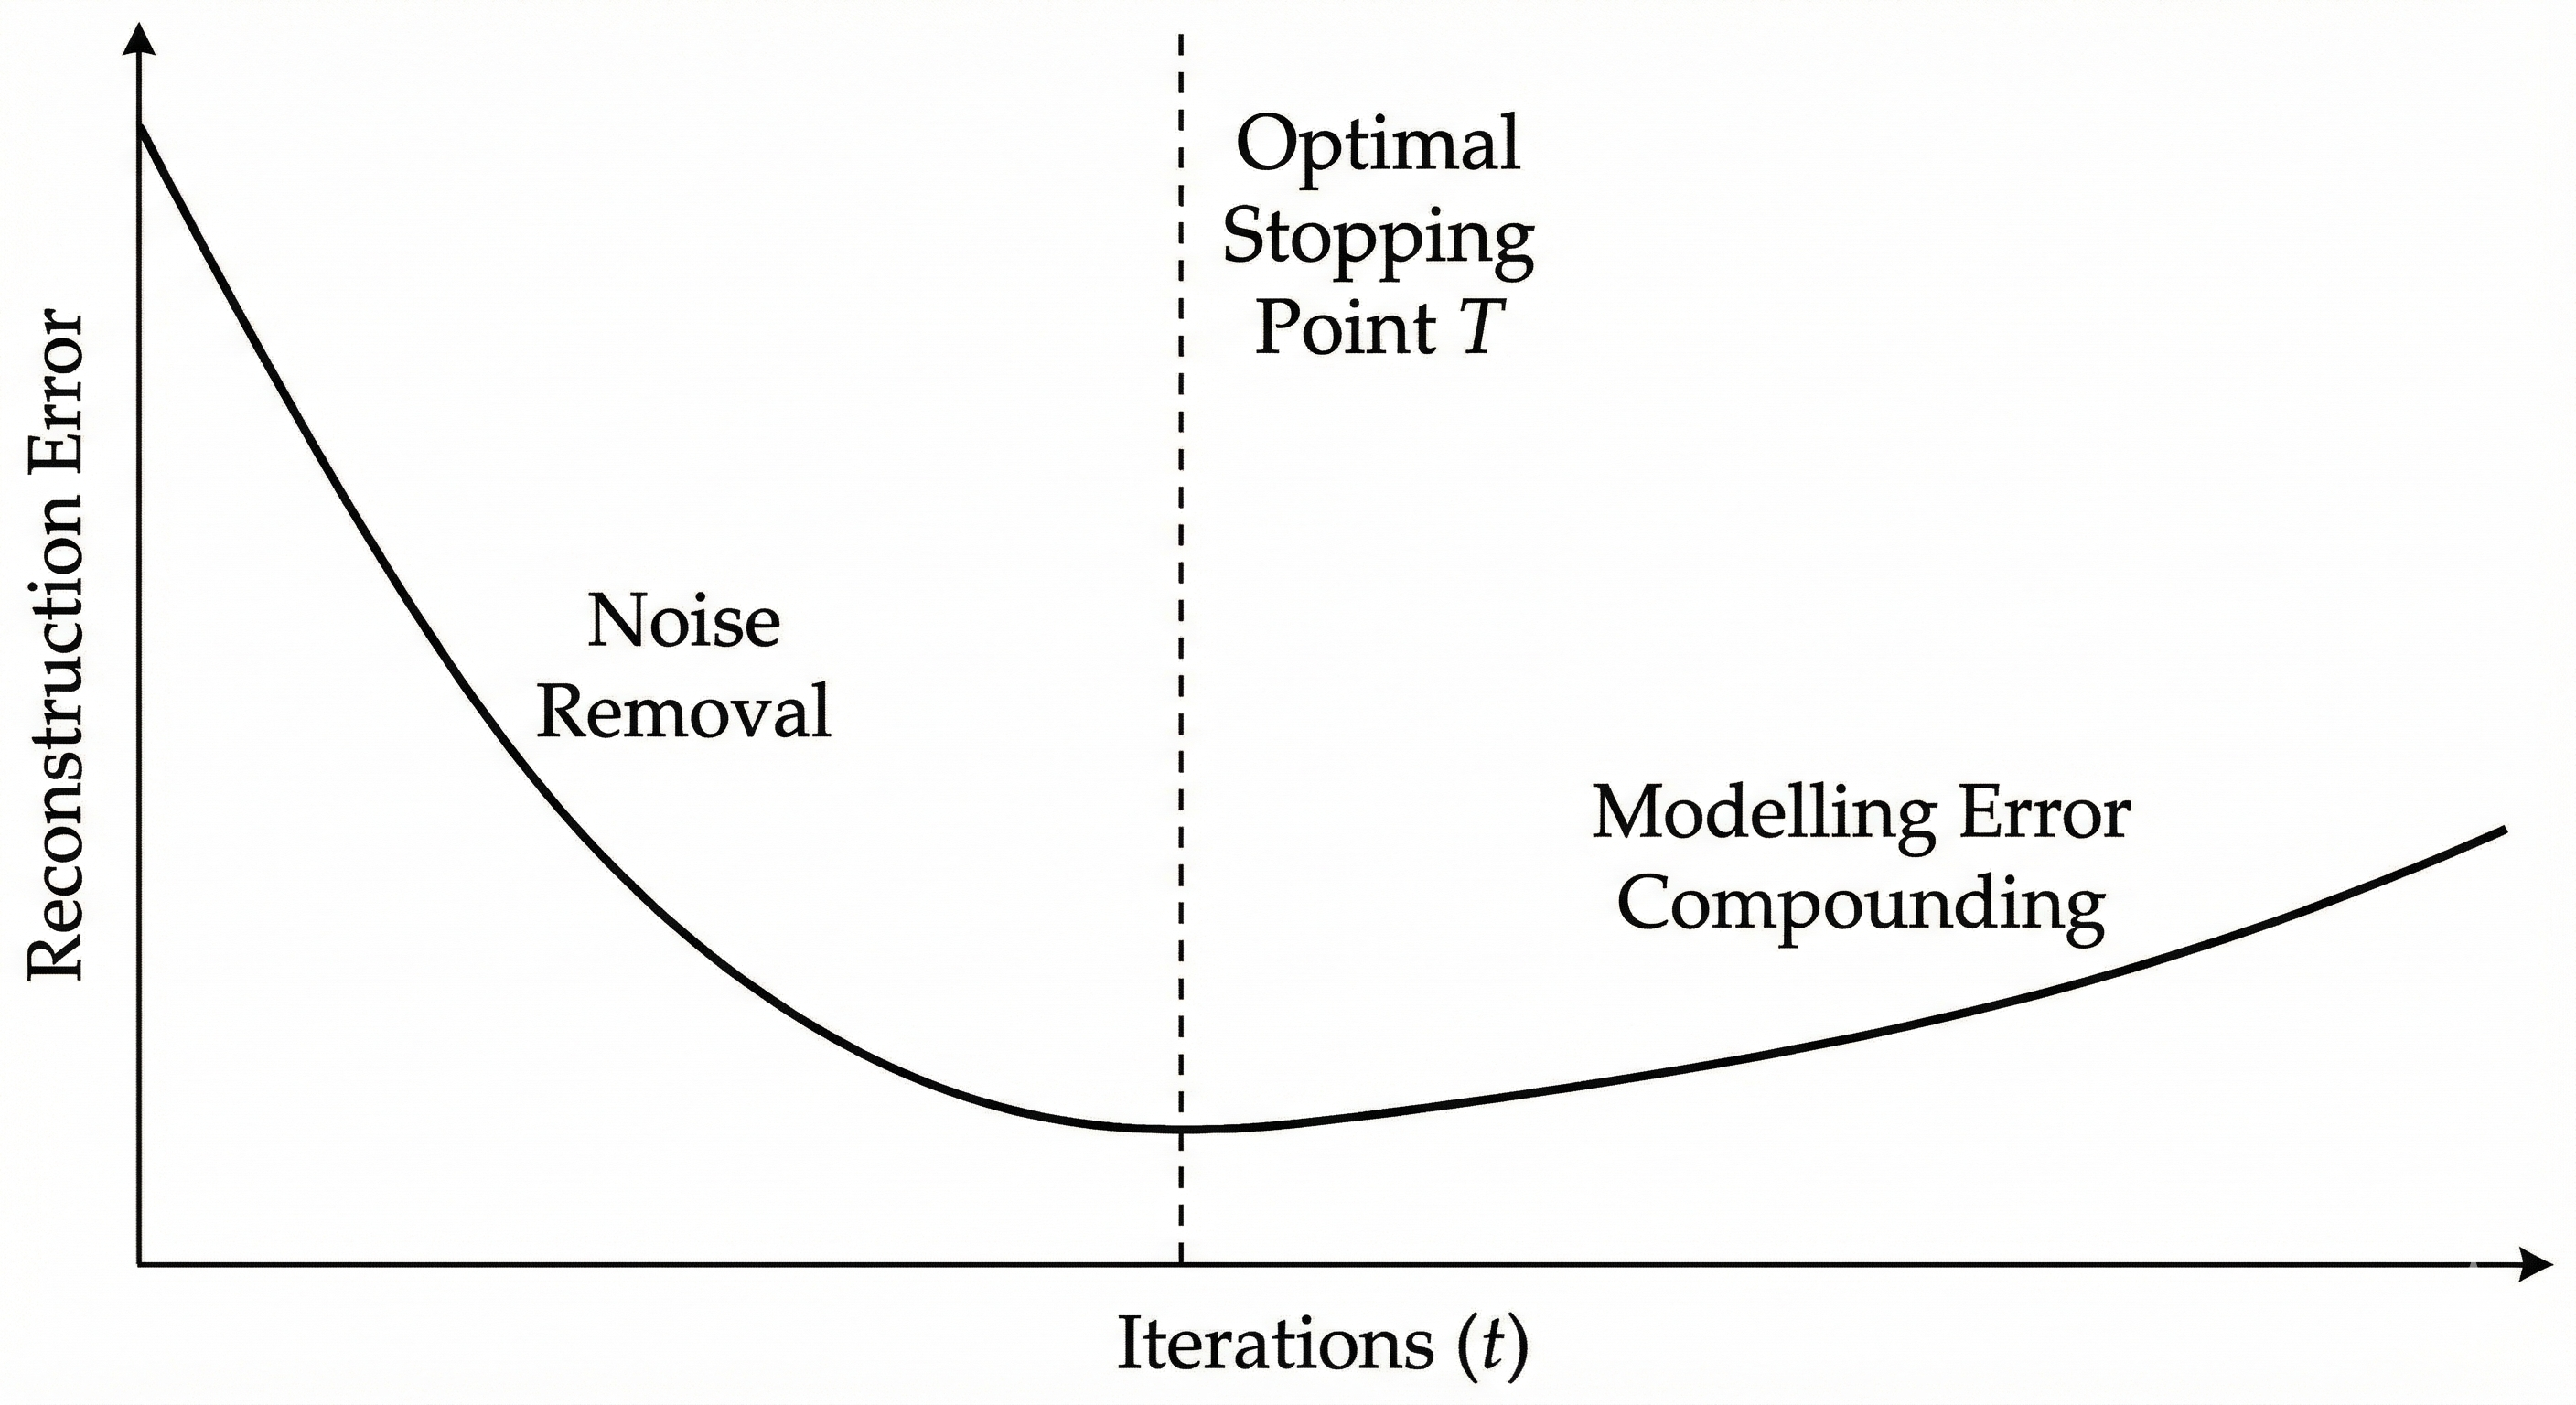
\includegraphics[width=\textwidth]{../Common_Images/varnetworks/convergence-trade-off.png}
            \end{figure}
        \end{column}
    \end{columns}
\end{frame}

\begin{frame}{Visualising the Paradox in TV-$L^2$ Denoising}
    \begin{figure}[htpb]
        \centering
        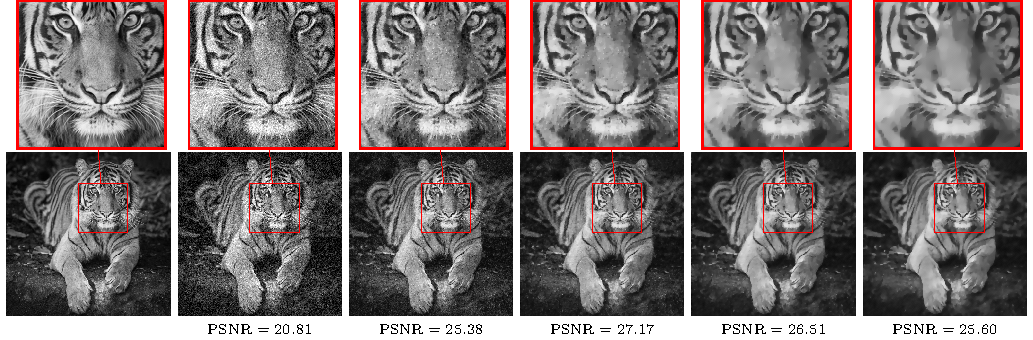
\includegraphics[width=0.9\textwidth]{../Common_Images/varnetworks/fig2.pdf}
        \caption{From left to right: input image, noisy continuous image, and restored images after 13, 26, 39, and 52 iterations. Optimal fidelity peaks at 26 iterations; further steps introduce staircasing artifacts \cite{effland2020variational}.}
    \end{figure}
\end{frame}

\begin{frame}{Why Infinite Iterations Degrade Quality}
    This ``early stopping paradox'' persists even in modern Variational Networks.\vspace{1em}
    
    Because infinite unrolled iterations degrade reconstruction quality, ensuring an ideal ``finite depth'' for our VNs becomes strictly paramount. 
    \vspace{1em}
    
    But how do we determine this stopping point rigorously, rather than relying on arbitrary hyperparameters or heuristic early stopping rules?
\end{frame}

\section{Stopping Time as a Continuous Control Parameter}

\begin{frame}{Moving Away from Heuristics}
    Rather than treating the architectural number of unrolled layers $T$ as a fixed hyperparameter, we can formulate Variational Networks seamlessly as a \textbf{continuous optimal control problem}.\vspace{1em}
    
    By doing so, the stopping time $T$ acts directly as an \emph{explicit, learnable control parameter} alongside the network weights $\Theta$.
\end{frame}

\begin{frame}{Time-Reparameterisation Technique}
    We define the state equation as the continuous gradient flow of the Variational Network energy functional. 
    
    To push the stopping time $T$ directly into the system dynamics, we employ a time-reparameterisation technique:
    $$x(t) = u(tT)$$
    
    This elegantly maps the integration bounds to exactly $t \in (0, 1)$, regardless of the actual duration $T$.
\end{frame}

% \begin{frame}{The Autonomous State ODE}
%     Applying this reparameterisation, the autonomous state ODE takes the generalised form:
    
%     $$ \frac{d}{dt}x(t) = T \mathcal{F}(x(t), \Theta) = T \left( -K^*(Kx(t) - f^\delta) - \sum_{k=1}^{N_D} (D_k)^\top \rho_k'\left(D_k x(t)\right) \right) $$
    
%     with the initial condition $x(0) = u_0$.
%     \vspace{1em}
    
%     Notice that $T$ acts as a scalar multiplier scaling the entire velocity vector field.
% \end{frame}

\begin{frame}{The Autonomous State ODE}
    Applying this reparameterisation, the autonomous state ODE takes the generalised form:
    
    \pause
    % Color-coding T in uclred and Theta in uclblue
    $$ \frac{d}{dt}x(t) = {\color{uclred}T} \mathcal{F}(x(t), {\color{uclblue}\Theta}) = {\color{uclred}T} \left( -K^*(Kx(t) - f^\delta) - \sum_{k=1}^{N_D} (D_k)^\top \rho_k'\left(D_k x(t)\right) \right) $$
    
    with the initial condition $x(0) = u_0$. \pause
    \vspace{1em}
    
    \begin{block}{Geometric Interpretation}
    Notice that ${\color{uclred}T}$ acts as a scalar multiplier scaling the \textbf{entire velocity vector field} evaluated by the network parameters ${\color{uclblue}\Theta}$.
    \end{block}
\end{frame}

\begin{frame}{The New Trajectory Cost Functional}
    Our optimal control challenge is now twofold: we seek to find the \textbf{optimal scalar stopping time $T$} and the \textbf{neural network parameters $\Theta$}.
    \vspace{1em}
    
    We aim to minimise the discrepancy between the final evaluated state at the mapped terminal time $t=1$ and the exact ground truth $u^\dagger$:
    
    $$ \mathcal{J}(x(1)) = \frac{1}{2}\|x(1) - u^\dagger\|_2^2 $$
\end{frame}

\begin{frame}{Trajectory Topology}
    \begin{figure}[htpb]
        \centering
        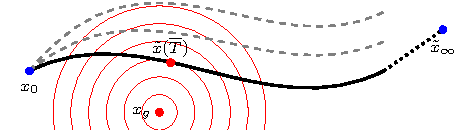
\includegraphics[width=0.65\textwidth]{../Common_Images/varnetworks/fig3.pdf}
        \caption{Schematic of a continuous state trajectory. The optimal control objective seeks the exact stopping time $\overline{T}$ where the trajectory is tangentially closest to the ground truth $x_g$, avoiding the mathematically stationary trap sink $\tilde{x}_\infty$ \cite{effland2020variational}.}
    \end{figure}
\end{frame}

\section{Optimality Conditions for Network Depth}

\begin{frame}{Building the Lagrangian for Depth}
    In direct analogy to Lecture 1, we now write the constrained optimal control problem explicitly as
    
    $$\min_{x,\Theta,{\color{uclred}T}}\;\mathcal{J}(x(1))=\frac{1}{2}\|x(1)-u^\dagger\|_2^2 \, . $$
    
    subject to
    $$\frac{d}{dt}x(t)-{\color{uclred}T}\,\mathcal{F}(x(t),\Theta)=0,\quad x(0)=u_0,\quad t\in(0,1].$$
    
    We introduce the adjoint state $p(t)$ and form the Lagrangian
    $$\mathcal{L}(x,p,\Theta,{\color{uclred}T})=\frac{1}{2}\|x(1)-u^\dagger\|_2^2+\int_0^1\!\left\langle p(t),\frac{d}{dt}x(t)-{\color{uclred}T}\,\mathcal{F}(x(t),\Theta)\right\rangle dt.$$
\end{frame}

% \begin{frame}{First-Order Optimality for Network Depth}
%     By evaluating the variation of the Lagrangian strictly with respect to the scalar horizon multiplier $T$, we recover a rigorous first-order necessary condition:
    
%     \begin{theoremblock}{Optimality Condition for $T$}
%     $$ \int_0^1 \left\langle p(t), \frac{d}{dt}x(t) \right\rangle \, dt = 0 $$
%     \end{theoremblock}
    
%     The continuous adjoint state $p(t)$ solves an associated backward-time ODE, initialised via the terminal condition $p(1) = x(1) - u^\dagger$.
% \end{frame}

\begin{frame}{First-Order Optimality for Network Depth}
    \only<1>{We differentiate $\mathcal{L}$ with respect to the scalar horizon ${\color{uclred}T}$ to obtain
    $$\partial_{\color{uclred}T}\mathcal{L}=-\int_0^1\left\langle p(t),\mathcal{F}(x(t),\Theta)\right\rangle dt.$$}
    At an optimum, $\partial_{\color{uclred}T}\mathcal{L}=0$, we observe
    $$\int_0^1\left\langle p(t),\mathcal{F}(x(t),\Theta)\right\rangle dt=0.$$ 
    Using $\frac{d}{dt}x(t)={\color{uclred}T}\,\mathcal{F}(x(t),\Theta)$ (and ${\color{uclred}T}>0$), this is equivalent to
    \begin{theoremblock}{Optimality Condition for ${\color{uclred}T}$}\vspace{-0.15cm}
    $$ \int_0^1 \left\langle p(t), \frac{d}{dt}x(t) \right\rangle \, dt = 0. $$
    \end{theoremblock}
    \vspace{-0.1cm}
    \only<2->{The corresponding adjoint equation is
    $$-\frac{d}{dt}p(t)= {\color{uclred}T}\left(\partial_x\mathcal{F}(x(t),\Theta)\right)^*p(t),\qquad p(1)=x(1)-u^\dagger.$$}
\end{frame}

% \begin{frame}{Interpreting the Condition: Structural Orthogonality}
%     What does this equation actually mean physically?
%     \vspace{1em}
    
%     It elegantly states that at the continuous global minimum of stopping time $T$, the integral product between the network's forward ODE velocity ($\frac{d}{dt}x$) and the adjoint error gradient field ($p$) must be perfectly \textbf{structurally orthogonal} \cite{effland2020variational}.
% \end{frame}

\begin{frame}{Interpreting the Condition: Structural Orthogonality}
    What does the optimality condition for ${\color{uclred}T}$ actually mean physically?
    \vspace{1em}
    
    \begin{columns}[T] % Align columns at the top
        \begin{column}{0.55\textwidth}
            It elegantly states that at the continuous global minimum of stopping time ${\color{uclred}T}$
            \vspace{0.5em}
            
            \begin{itemize}
                \item<2-> The network's forward ODE velocity ($\frac{d}{dt}x$)
                \item<3-> And the adjoint error gradient field ($p$)
            \end{itemize}
            \vspace{0.5em}
            
            \uncover<4->{must be perfectly \textbf{structurally orthogonal} \cite{effland2020variational}.}
        \end{column}
        
        \begin{column}{0.4\textwidth}
            % This uses TikZ (already in your preamble) to draw a simple geometric representation
            \uncover<4->{
                \begin{figure}
                    \centering
                    \begin{tikzpicture}[scale=1.2]
                        % Draw axes/vectors
                        \draw[->, thick, uclblue] (0,0) -- (2,0) node[right] {$\frac{d}{dt}x$};
                        \draw[->, thick, darkgreen] (0,0) -- (0,2) node[above] {$p(t)$};
                        % Draw right angle square
                        \draw (0.3,0) -- (0.3,0.3) -- (0,0.3);
                        % Add dot product note
                        \node at (1, 1) {$\left\langle p, \frac{d}{dt} x \right\rangle = 0$};
                    \end{tikzpicture}
                \end{figure}
            }
        \end{column}
    \end{columns}
\end{frame}

\begin{frame}{Visualising the Optimality Condition}
    \begin{figure}[htpb]
        \centering
        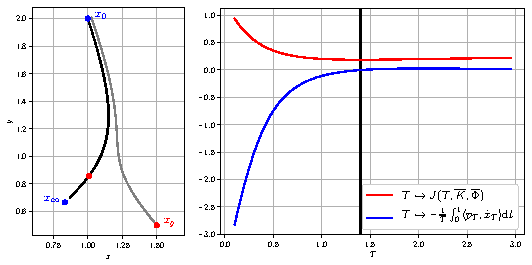
\includegraphics[width=0.85\textwidth]{../Common_Images/varnetworks/fig4.pdf}
        \caption{The continuous first-order optimality objective strictly evaluates to $0$ precisely at the optimal halting time corresponding to the global $L^2$ trajectory metric \cite{effland2020variational}.}
    \end{figure}
\end{frame}

\begin{frame}{Second-Order Conditions}
    To guarantee that this optimal time $T$ acts stably as a local minimum (verifying that increasing depth further will natively harm performance), one evaluates second-order conditions.
    \vspace{1em}
    
    \begin{itemize}
        \item We require a strict second-order sufficient gradient condition ensuring strict positivity across the local curvature field.
        \item By jointly optimising parameters $\Theta$ alongside $T$, the continuous network architecture dynamically derives its optimal depth natively from structural data gradients!
    \end{itemize}
\end{frame}

\section{Nonlinear Spectral Dynamics \& Conclusion}

\begin{frame}{Connection to Discretised Static Networks}
    We can easily derive standard neural architectures simply by running explicit numerical integration templates on our continuous Variational framework. 
    \vspace{1em}
    
    A forward Euler time discretisation across a uniform set of nodes with step sizes $\Delta t = T/S$ gives:
    $$ x_{s+1} = x_s + \frac{T}{S} \mathcal{F}(x_s, \Theta) $$
    
    These are functionally equivalent to deep Residual Networks where parameters $\Theta$ are static (shared identically) across layers, commonly termed \textbf{Static Variational Networks}.
\end{frame}

\begin{frame}{Nonlinear Spectral Dynamics}
    Why does the network flow formally improve the imaging structures before halting safely, rather than indiscriminately destroying the picture?
    \vspace{1em}
    
    Effland et al. analysed the gradient of the highly-parameterised field-of-experts model specifically via \textbf{nonlinear eigenvalue problems}:
    $$ \sum_{k=1}^{N_D} D_k^\top \rho_k'(D_k v) = \lambda v $$
\end{frame}

\begin{frame}{Understanding the Eigenvalues}
    Extracting the generalised eigenfunctions $v_j$ corresponding to various eigenvalues $\lambda_j$ unravels exactly what the discretised layers dynamically evaluate.
    \vspace{1em}
    
    The contraction factor applied to an eigenfunction at each layer maps to $(1 - \lambda_j \frac{T}{S}) v_j$.
    
    \begin{itemize}
        \item \textbf{High-frequency noise:} Produces very \textbf{large} eigenvalues (heavy damping / sharp contraction).
        \item \textbf{Structural boundaries/textures:} Produce exceedingly \textbf{small} eigenvalues near $0$ (contraction factor $\approx 1$, structures are preserved).
    \end{itemize}
\end{frame}

\begin{frame}{Eigenpairs in Action (I)}
    \begin{figure}[htpb]
        \centering
        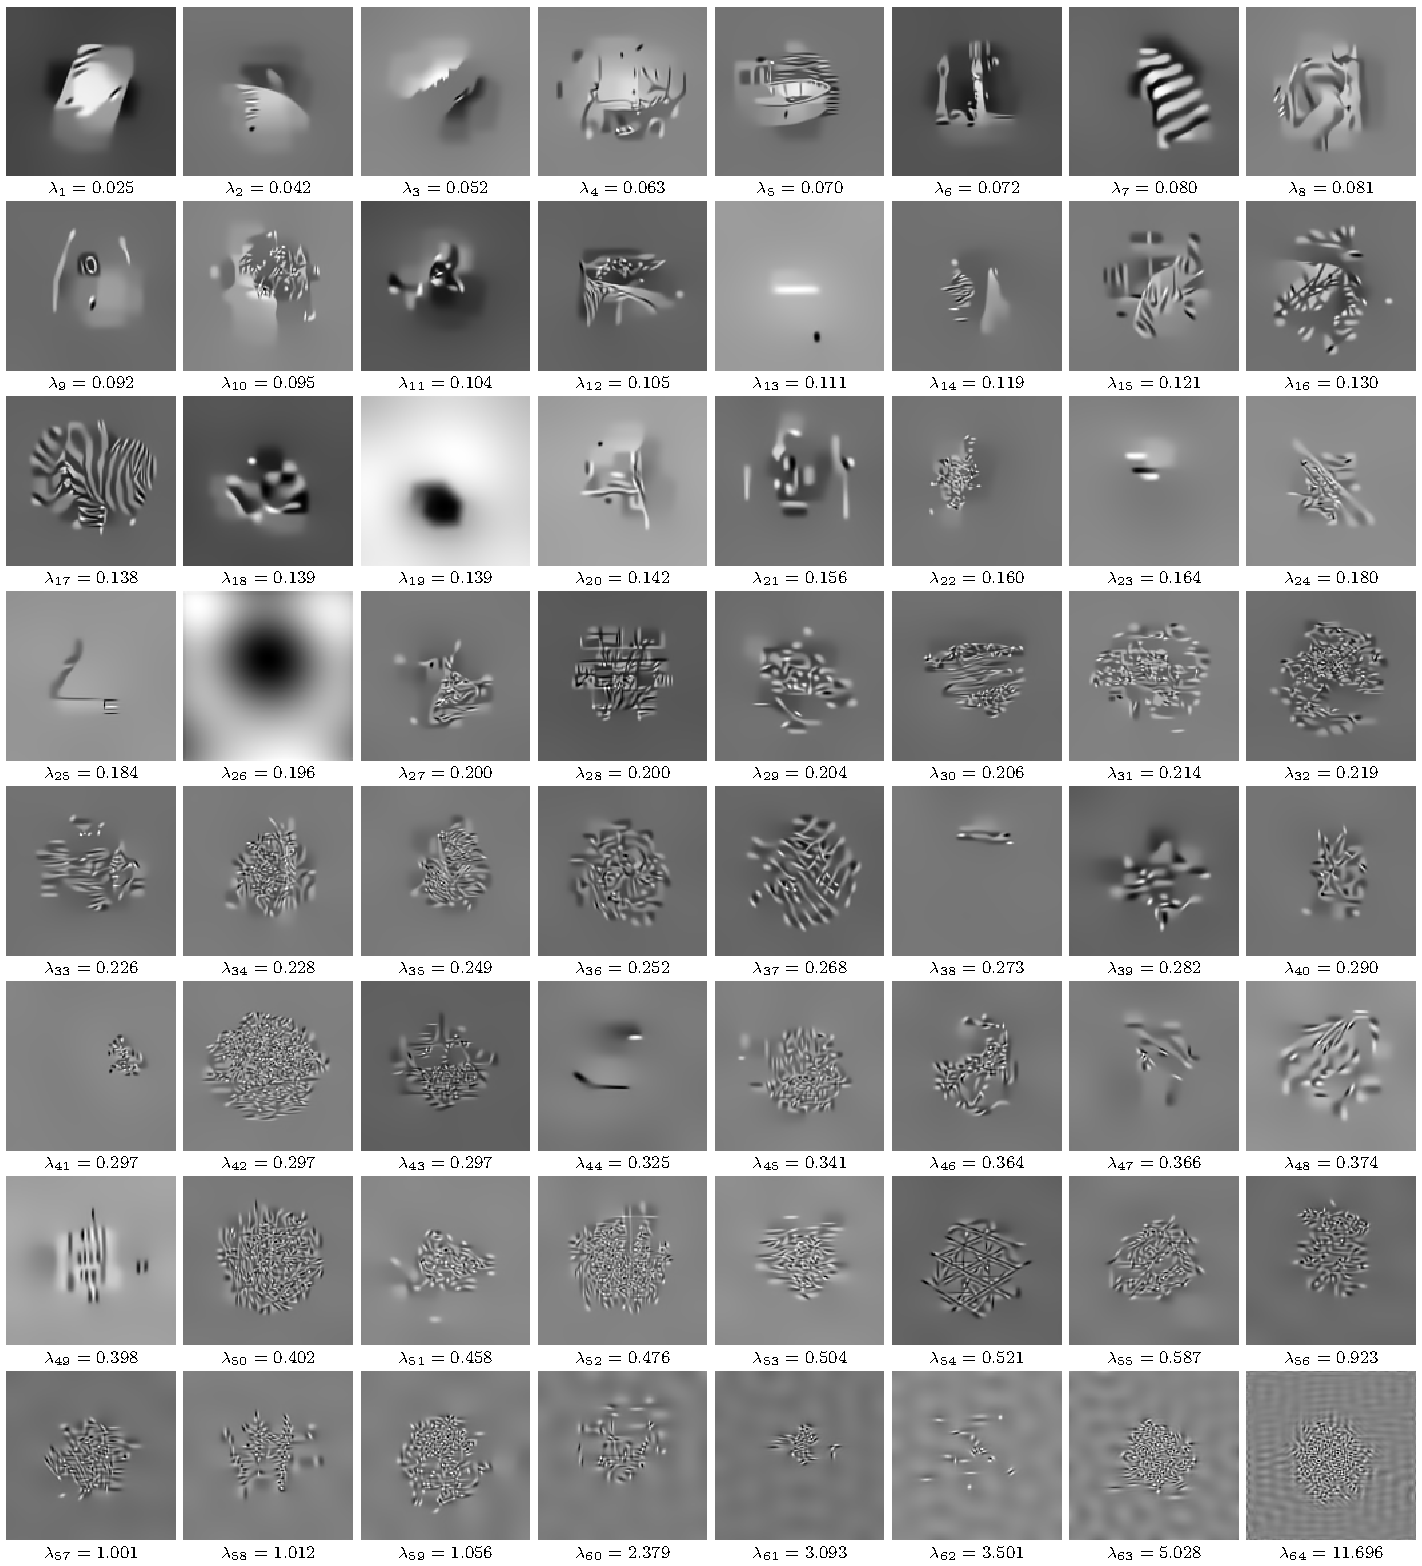
\includegraphics[trim=0 {2.2\textheight} 0 0, clip, height=0.80\textheight, keepaspectratio]{../Common_Images/varnetworks/fig13.pdf}
        {\captionsetup{font=scriptsize}\caption{Top panel: low $\lambda$ align with large-scale structures and are less attenuated \cite{effland2020variational}.}}
    \end{figure}
\end{frame}

\begin{frame}{Eigenpairs in Action (II)}
    \begin{figure}[htpb]
        \centering
        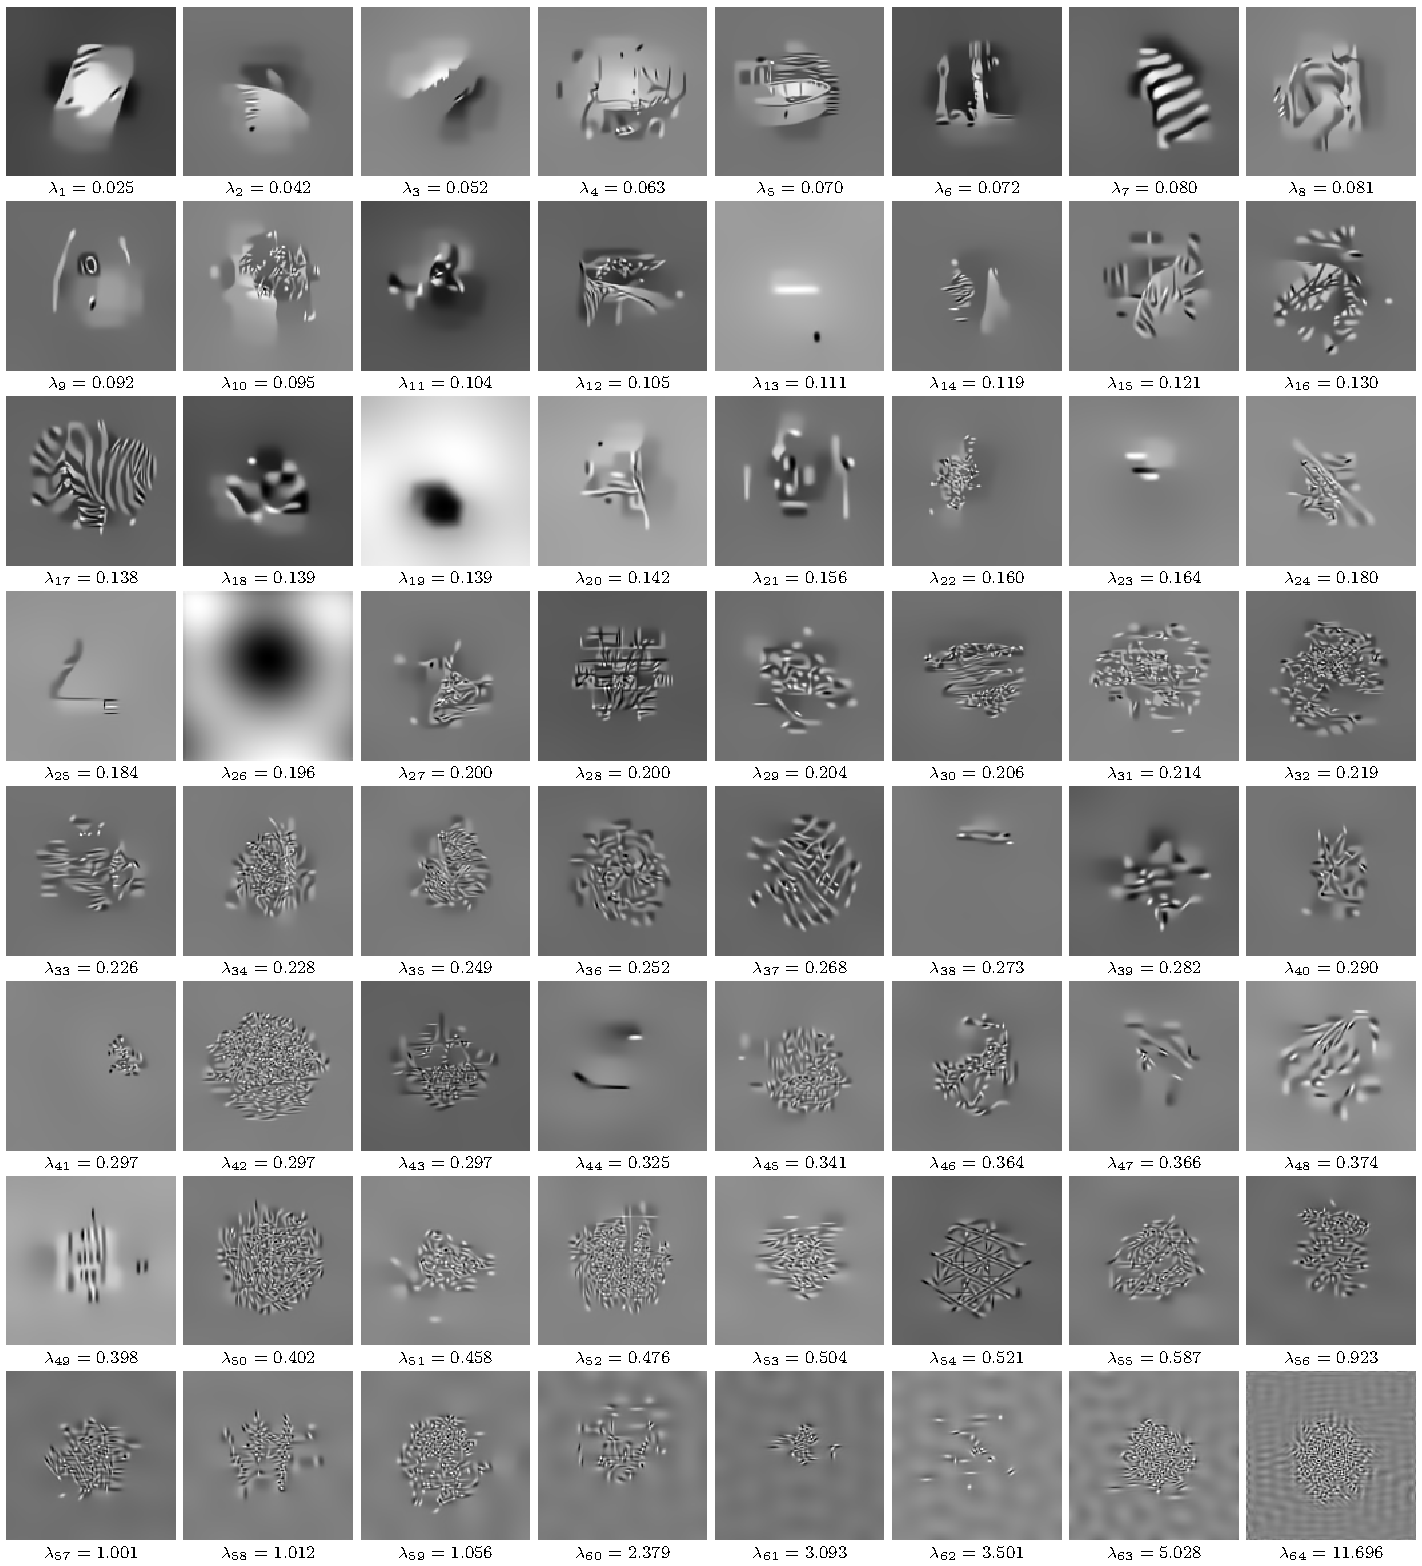
\includegraphics[trim=0 {1.1\textheight} 0 {1.1\textheight}, clip, height=0.80\textheight, keepaspectratio]{../Common_Images/varnetworks/fig13.pdf}
        {\captionsetup{font=scriptsize}\caption{Middle panel: transition from structural modes to finer-scale content \cite{effland2020variational}.}}
    \end{figure}
\end{frame}

\begin{frame}{Eigenpairs in Action (III)}
    \begin{figure}[htpb]
        \centering
        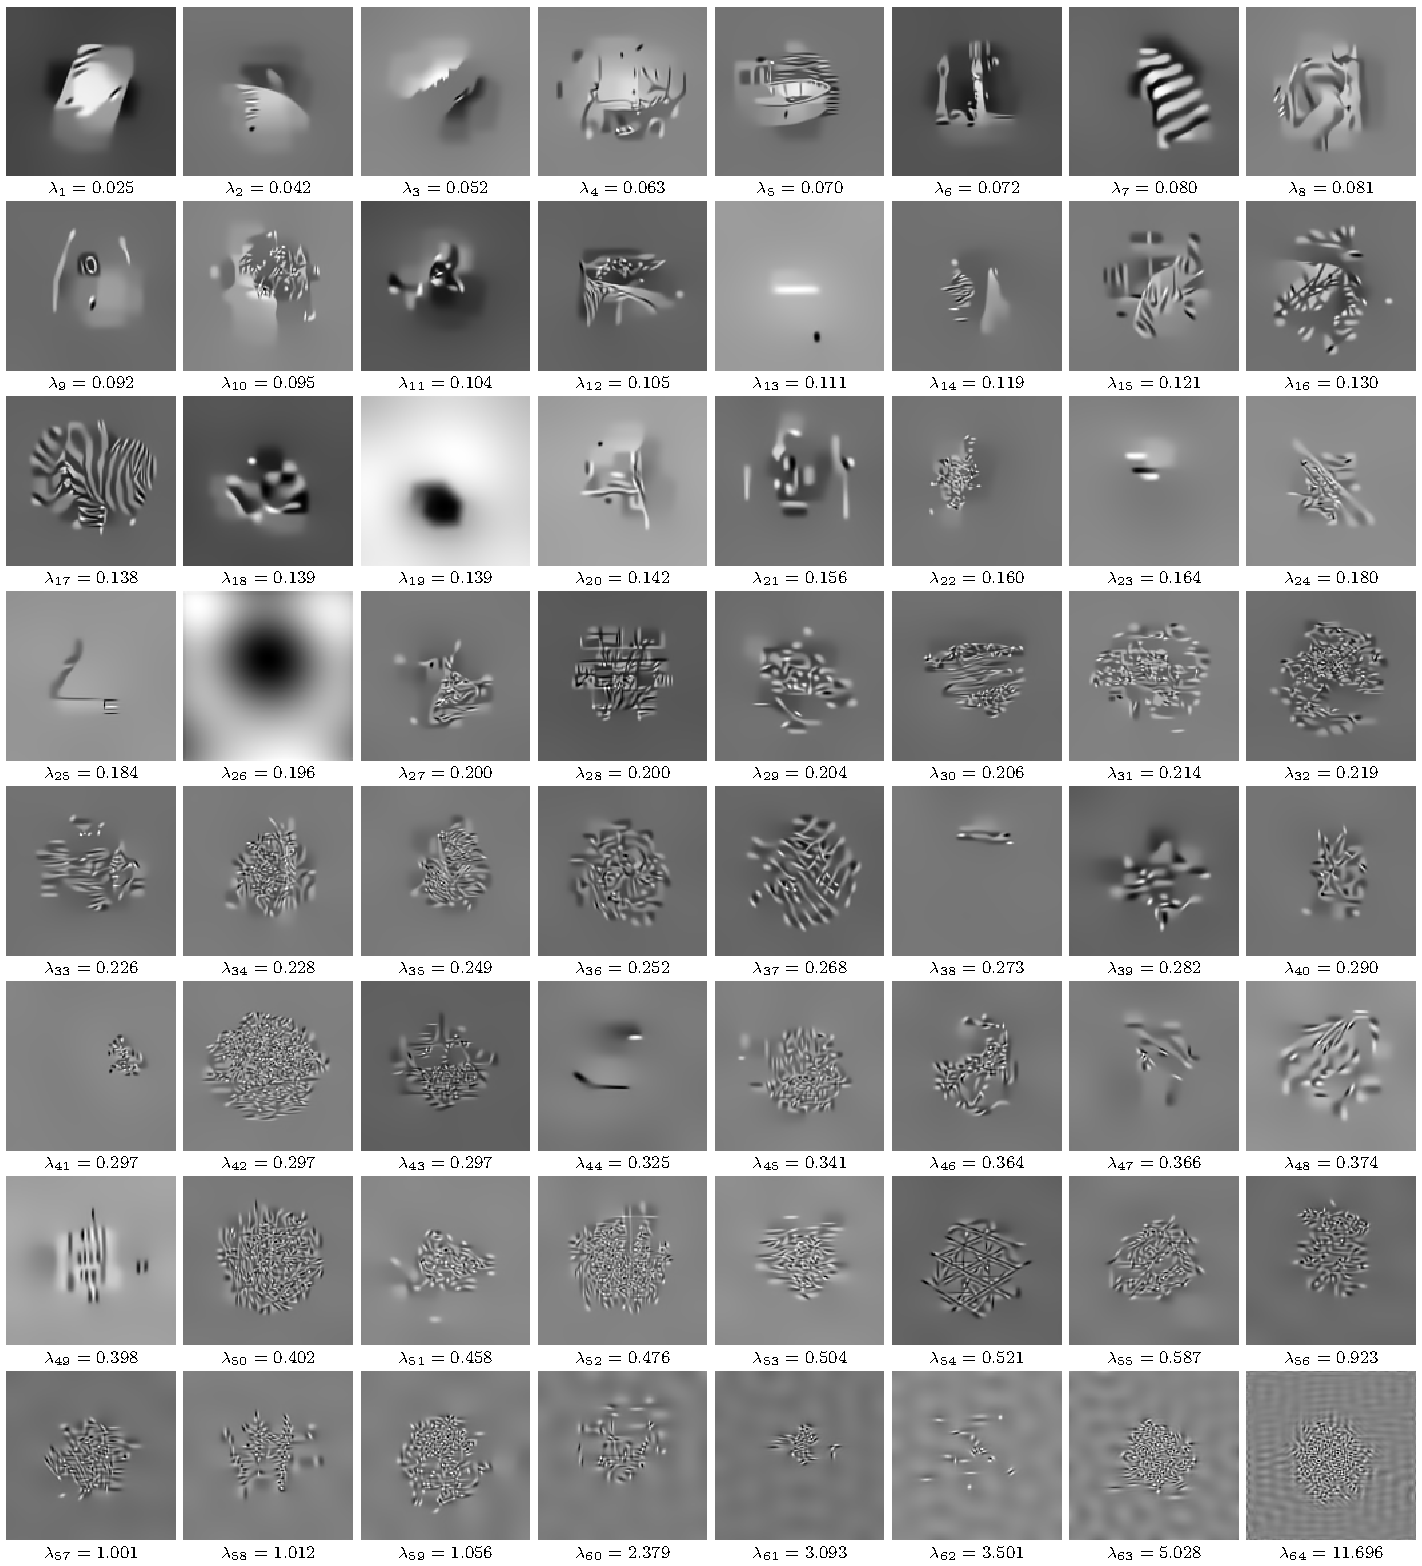
\includegraphics[trim=0 0 0 {2.2\textheight}, clip, height=0.80\textheight, keepaspectratio]{../Common_Images/varnetworks/fig13.pdf}
        {\captionsetup{font=scriptsize}\caption{Bottom panel: high eigenvalues mainly capture granular noisy structures \cite{effland2020variational}.}}
    \end{figure}
\end{frame}

\begin{frame}{Chapter Summary: Unifying Paradigms}
    In this chapter, we executed a profound perspective shift, unifying multiple paradigms:
    
    \begin{enumerate}
        \item \textbf{Continuous ODEs:} Reframed deep Residual Networks and Unrolled Algorithms as continuous dynamical systems.
        \item \textbf{Optimal Control:} Transformed the supervised learning problem into deriving an optimal control trajectory via the Lagrangian and Hamiltonian (Pontryagin's Minimum Principle).
        \item \textbf{Physics-Based Priors:} Reversed the perspective to build Variational Networks from discretised physical energy functionals.
        \item \textbf{Dynamic Depth:} Resolved the Early Stopping Paradox by treating the network stopping time $T$ as a mathematically rigorous, learnable optimal control parameter.
    \end{enumerate}
\end{frame}

\begin{frame}[allowframebreaks]{References}
    \bibliographystyle{abbrv}
    \bibliography{../../Lecture_Notes/references}
\end{frame}

\end{document}